\documentclass[conference]{IEEEtran}
\usepackage{cite}
\ifCLASSINFOpdf
   \usepackage[pdftex]{graphicx}
 \fi
\usepackage[cmex10]{amsmath}
\usepackage{tikz}
\usepackage{hyperref}
\usepackage{caption} 
\captionsetup[table]{skip=10pt}
\usetikzlibrary{matrix,chains,positioning,decorations.pathreplacing,arrows}
\usepackage{amsmath}
\usepackage{float}
\usepackage{booktabs}
\IEEEoverridecommandlockouts
%s\hyphenation{op-tical net-works semi-conduc-tor}
\title{Movie Recommendations Using \\ Low-dimensional Codes}
\author{
\IEEEauthorblockN{Christopher Curro, David Katz, Harrizon Zhao}
\IEEEauthorblockA{The Cooper Union\\
Electrical Engineering
}
}
\begin{document}
\maketitle
\global\csname @topnum\endcsname 0
\global\csname @botnum\endcsname 0
\begin{abstract} 

We present a movie recommendation system that finds a weighted set of nearest
neighbors to an arbitrary desired movie based on user specified interests in a
latent space learned by an autoencoder. We learn a low-dimensional
representation to make recommendations in from a much larger feature space
consisting of approximately one thousand tags and their relevancies to about
ten thousand movies. 

\end{abstract} 
\section{Introduction} 

Movie recommendation is complex task that generally involves high dimensional
feature spaces; a common approach today is the collaborative filtering
approach \cite{ekstrand2011collaborative,good1999combining,koren2009matrix}.
The collaborative filtering approach is powerful because successfully reduces
a complex high-dimensional feature space into a rich low-dimensional latent
space. We aim to present an alternative approach to generating a rich low-dimensional latent space capable of producing high quality movie
recommendations based on nearest neighbor approach where the queried sample is
determined by user input. We work with the dataset created by Vig et al.
\cite{vig2012tag}. This dataset provides a approximately ten thousand movies each with relevance weightings for approximately one thousand tags.

\subsection{Autoencoders}
\begin{figure}
\centering
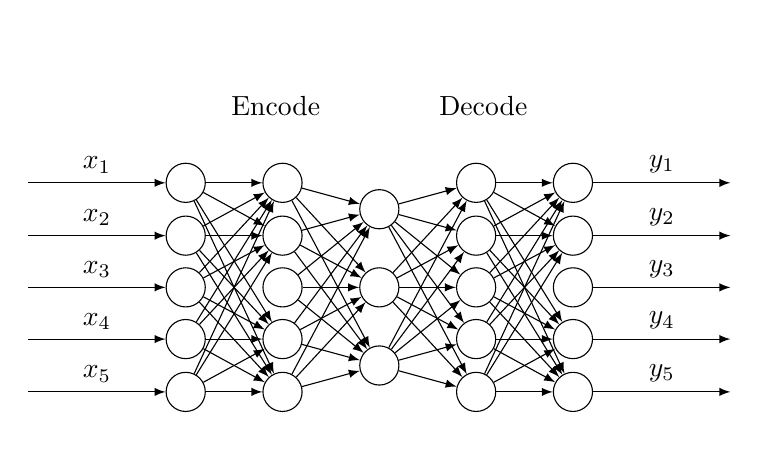
\begin{tikzpicture}[
plain/.style={
  draw=none,
  fill=none,
  },
net/.style={
  matrix of nodes,
  nodes={
    draw,
    circle,
    inner sep=5pt
    },
  nodes in empty cells,
  column sep=-0.5cm,
  row sep=-5pt
  },
>=latex
]
\matrix[net] (mat)
{
|[plain]| \parbox{1.3cm}{\centering \hfill} & |[plain]| \parbox{1.3cm}{Encode} & |[plain]| \parbox{1.3cm}{\centering \hfill}  & |[plain]| \parbox{1.3cm}{\raggedleft Decode} & |[plain]| \parbox{1.3cm}{\centering \hfill} \\
& & |[plain]| & & &|[plain]|\\
|[plain]| & |[plain]|& & |[plain]|\\
& &|[plain]| & & &|[plain]|\\
|[plain]| & |[plain]| \\
&& & & &|[plain]|\\
|[plain]| &|[plain]|& |[plain]| \\
& & |[plain]| & & &|[plain]|\\
|[plain]|&|[plain]| & & |[plain]|\\
& & |[plain]| & & &|[plain]|\\
};
\foreach \ai [count=\mi ]in {2,4,...,11}
  \draw[<-] (mat-\ai-1) -- node[above] {$x_\mi$} +(-2cm,0);

% Middle lines  
\foreach \ai in {2,4,...,10}
{\foreach \aii in {2,4,8,10}
  \draw[->] (mat-\ai-1) -- (mat-\aii-2);
}

\foreach \ai in {2,4,...,10}
{\foreach \aii in {3,6,9}
  \draw[->] (mat-\ai-2) -- (mat-\aii-3);
}
% last three lines
\foreach \ai in {2,4,6,8,10}
{
\foreach \aii in {3,6,9}
  \draw[->] (mat-\aii-3) -- (mat-\ai-4);
}

\foreach \ai in {2,4,...,10}
{\foreach \aii in {2,4,8,10}
  \draw[->] (mat-\ai-4) -- (mat-\aii-5);
}


\foreach \ai [count=\mi ]in {2,4,...,11}
  \draw[->] (mat-\ai-5) -- node[above] {$y_\mi$} +(2cm,0);
\end{tikzpicture}
\caption{
A simple autoencoder with a two layer encoder/decoder pair. This autoencoder
would code a five dimensional space into a three dimensional space. Each neuron represents a weighted sum passed through an activation function.
}
\label{autoenc}
\end{figure}

An autoencoder is a particular type of neural network. A neural network is a computational graph where nodes can be
defined in the form: 
\begin{equation}
\mathbf{y} = f\left(W\mathbf{x} + \mathbf{b}\right)
\label{dense}
\end{equation}
Where $\mathbf{x}$ is an input vector, $W$ and $b$ are parameters that define a
linear relationship, and $f(\cdot)$ is an activation function. The activation
function is generally a non-linear function so each node in the graph can
perform a non-linear mapping from $\mathbf{x}$ to $\mathbf{y}$.

Nodes can be connected successively to one another in a feed-forward fashion to
create increasingly complex representations of the input data. Nodes in these
networks are generally referred to as layers, and can be represented
diagrammatically as in Figure \ref{autoenc}. 

Figure \ref{autoenc} in particular shows an autoencoder. Unlike an ordinary
neural network an autoencoder contains a bottleneck in the middle. It is this
bottleneck that creates the rich dimensionality reduction power of an
autoencoder. This bottleneck essentially splits the network into two stages:
the encoder stage and the decoder stage. We interpret the autoencoder as
having two stages because we optimize the learned parameters of the
autoencoder to minimize the reconstruction error at the output of the decoder.
By following this objective and applying other constraints, such as a sparsity constraints, rich coding schemes can be achieved at the bottleneck.

\subsection{Nearest Neighbors Recomendations}
After selecting a latent feature space in order to find recommendations for a query, a recommendation engine must perform a nearest neighbors query.  The movies with the closest distance to the user's input or latent features are selected as recommendations \cite{sarwar2001item}.

For multi-dimensional spaces, the only method which is guaranteed to return exact nearest neighbors is a linear search \cite{flann_pami_2014}.  This becomes unfeasible with larger datasets with many users.  For this reason, recommendation systems tend to use approximate nearest neighbors methods, as there is little consequence for recommending a set of movies which are close to the best recommendations rather than the exact best.  To do so, an index is constructed on the dataset once.  Each query applies this index will only search a small subset of the entire dataset but will still return close to the best results.

Typically for relatively low dimensional spaces the Euclidean distance metric is used.  However, to handle the constraint of user specified dimension relevance we used a modified Euclidean distance metric shown in Equation \ref{eq:distmet}.  The x and y represent two movies, while v represents the user specified weight on each dimension.  Since v is normalized to have a sum of 1, when v is uniform this metric is equivalent to Euclidean distance.
\begin{equation}
\label{eq:distmet}
distance(x,y,v) = \sqrt{\sum\limits_{i=1}^D ((x_i - y_i) \times v_i \times D)^2}
\end{equation}


\section{System Description}

\subsection{Autoencoder}
The autoencoder we created to perform the dimensionality reduction encodes a
length 1128 vector down to length 10 code. This is performed with a single
hidden-layer encoder and a single-hidden layer decoder. All of the neurons are
hyperbolic tangent neurons. These were selected over sigmoidal neurons because
their derivatives are symmetric around zero and therefore they learn their
parameters more quickly \cite{sibi2013analysis}. The encoding and decoding
stages shared the same number of neurons in each layer. Both stages were
constructed from two layers consisting of 1128 neurons and one layer
consisting  of 10 neurons. (This accounting includes the unweighted input neurons for both the encoder and decoder.)

We implemented and trained the present autoencoder with the Torch 7
\cite{collobert2011torch7} framework; the computation was accelerated through
the use of an Nvidia Tesla K40. We selected the mean squared reconstruction
error as our criterion and used Nesterov accelerated gradient descent
\cite{nesterov2007gradient} to optimize it.
\subsection{Recomendations}
Since this dataset is relatively small and we do not expect a large number of users, a linear search for the top k movies is feasible.  However, to scale to a larger userbase and a larger dataset, and approximate nearest neighbors index should be used.  While typical approximate nearest neighbors indexes are not adaptable to query specified dimension relevance.  \cite{davethesis} describes an efficient index for handling this type of nearest neighbor query.

\section{Results}

\section{Conclusion}

% \IEEEpeerreviewmaketitle

\raggedright
\bibliographystyle{IEEEtran}
\bibliography{bib}

\end{document}
